% This is a modified version of the tufte-latex book example in which the title page and the contents page resemble Tufte's
% VDQI book, using Kevin Godby's code from this thread at https://groups.google.com/forum/#!topic/tufte-latex/ujdzrktC1BQ.
% Taken from https://www.overleaf.com/5902299yxkgzs#/19519356/
\documentclass[nohyper]{tufte-book}
\usepackage{nameref}
\usepackage[utf8]{inputenc}
\usepackage[italian]{babel}
\usepackage{ragged2e}
\usepackage{hyperref}
\RequirePackage[utf8]{inputenc}
\RequirePackage[italian]{babel}
\usepackage{amsmath}
\usepackage{amsthm}
\usepackage{amsfonts}
\usepackage{xifthen}
%\usepackage{xparse}
%\usepackage{etoolbox}% http://ctan.org/pkg/etoolbox
%\usepackage[linktoc=all]{hyperref} % Per i collegamenti ipertestuali. [linktoc=all] mette i link nell'indice

% https://it.sharelatex.com/blog/2011/03/27/how-to-write-a-latex-class-file-and-design-your-own-cv.html

\newcommand{\frdx}{ \framebox[\width]{ $\Rightarrow$ } }
\newcommand{\frsx}{ \framebox[\width]{ $\Leftarrow$ } }
\newcommand{\hrar}{\hookrightarrow}
\newcommand{\opp}{\text{ oppure }}
\def\checkmark{\tikz\fill[scale=0.4](0,.35) -- (.25,0) -- (1,.7) -- (.25,.15) -- cycle;} 
\newcommand{\crossmark}{$\times$}

%mathbb mathcal mathfrak e mathbm per le lettere dell'alfabeto e anche mathbb per quelle greche
\def\mydeflett#1{\expandafter\def\csname bb#1\endcsname{\mathbb{#1}}
		\expandafter\def\csname c#1\endcsname{\mathcal{#1}}
		\expandafter\def\csname k#1\endcsname{\mathfrak{#1}}
		\expandafter\def\csname bl#1\endcsname{\mathbf{#1}}}
\def\mydefalllett#1{\ifx#1\mydefalllett\else\mydeflett#1\expandafter\mydefalllett\fi}
\mydefalllett ABCDEFGHIJKLMNOPQRSTUVWXYZ\mydefalllett

\def\mydeffrakmath#1{\expandafter\def\csname k#1\endcsname{\mathfrak{#1}}}
\def\mydefallfrak#1{\ifx#1\mydefallfrak\else\mydeffrakmath#1\expandafter\mydefallfrak\fi}
\mydefallfrak abcdefghijklmnopqrstuvwxyz\mydefallfrak

\def\mydefgreek#1{\expandafter\def\csname bl#1\endcsname{\text{\boldmath$\mathbf{\csname #1\endcsname}$}}}
\def\mydefallgreek#1{\ifx\mydefallgreek#1\else\mydefgreek{#1}%
   \lowercase{\mydefgreek{#1}}\expandafter\mydefallgreek\fi}
\mydefallgreek {Gamma}{Delta}{Theta}{Lambda}{Xi}{Pi}{Sigma}{Upsilon}{Phi}{Varphi}{Psi}{Omega}{alpha}{beta}{gamma}{delta}{epsilon}{varepsilon}{zeta}{eta}{theta}{iota}{kappa}{lambda}{mu}{nu}{xi}{omicron}{pi}{rho}{sigma}{tau}{upsilon}{phi}{varphi}{chi}{psi}{omega}\mydefallgreek

%\NewDocumentCommand{\de}{gg}{
%\IfNoValueTF{#1}
%		{\text{ d}}
%		{\IfNoValueTF{#2}	{\text{ d}#1}
%			{\frac{\text{d}#1}{\text{d}#2}}
%	}
%}

%\NewDocumentCommand{\dpar}{gg}{
%	\IfNoValueTF{#1}
%		{\partial}
%		{\IfNoValueTF{#2}	{\partial_{#1}}
%			{\frac{\partial {#1}}{\partial {#2}}}
%	}
%}


%nuovi comandi per svariate cose (alcune per evitare di scrivere
\newcommand{\sse}{\Leftrightarrow}
\newcommand{\Rar}{\Rightarrow}
\newcommand{\rar}{\rightarrow}
\newcommand{\ol}[1]{\overline{#1}}
\newcommand{\ot}[1]{\widetilde{#1}}
\newcommand{\oc}[1]{\widehat{#1}}
\newcommand{\tc}{\text{ t.c. }}
\newcommand{\nowlog}{ Senza perdità di generalità }
\newcommand{\wlogsupp}{ Senza perdità di generalità possiamo supporre }
\newcommand{\spa}{ Supponiamo per assurdo }

\newcommand{\norma}[1]{\mid\mid #1 \mid\mid}
\newcommand{\abs}[1]{\mid #1 \mid}
\newcommand{\scal}[2]{\langle #1 \mid #2 \rangle}
\newcommand{\floor}[1]{\lfloor #1 \rfloor}

\newcommand{\Ker}{\text{Ker }}
\newcommand{\Deg}{\text{deg }}
\newcommand{\Det}{\text{det }}
\newcommand{\Dim}{\text{dim }}
\newcommand{\End}{\text{End }}
\newcommand{\Rk}{\mbox{rk }}
\newcommand{\Tr}{\text{tr }}
\newcommand{\GL}{\text{GL}}
\newcommand{\Omeo}{\text{Omeo }}
\newcommand{\Fix}{\text{Fix }}
\newcommand{\Supp}{\text{Supp }}
\newcommand{\Span}{\text{Span }}
\newcommand{\Img}{\text{Im }}
\newcommand{\Id}{\text{Id}}

% Cusu-comandi
\newcommand{\sdR}{superficie di Riemann}
\newcommand{\quoziente}[2]{\left.\raisebox{.2em}{$#1$}\middle/\raisebox{-.2em}{$#2$}\right.}
\newcommand{\Lar}{\Leftarrow}
\newcommand{\lar}{\leftarrow}
\newcommand{\isom}{\simeq}

% Comando per plottare una curva algebrica
% Nell'ordine i parametri sono:
% 1. Equazione della curva (in due variabili)
% 2. xrange (in notazione [inizio:fine])
% 3. yrange (come sopra)
% DAMETTERE 4. opzioni (tipo se metterci la griglia o no)
\newcommand{\curvegraph}[3]{
    \begin{tikzpicture}
    \draw[very thin,color=gray] (-1.9,-3.9) grid (3.9,3.9);
    \draw[->] (-2,0) -- (4.2,0) node[right] {$x$};
    \draw[->] (0,-4.2) -- (0,4.2) node[above] {$y$};
    \draw plot[id=curve, raw gnuplot, smooth] function{
    f(x,y) = #1;
    set xrange #2;
    set yrange #3;
    set view 0,0;
    set isosample 1000,1000;
    set size square;
    set cont base;
    set cntrparam levels incre 0,0.1,0;
    unset surface;
    splot f(x,y);
    };
    \end{tikzpicture}
}

\sloppy



% Manteniamo le note a piè di pagina nella stessa pagina
\interfootnotelinepenalty=10000
\makeatletter
\renewcommand\@makefntext[1]{\nohyphenation\justify\@makefnmark#1}
\makeatother

% Book metadata
\title{Curve Ellittiche e Modulari}
\date{Note di un corso del Prof. Umberto Zannier}
\author[]{Classe del Terzo Anno SNS}
\publisher{Versione del \dateitalian\today}

% Just some sample text
\usepackage{lipsum}

% For nicely typeset tabular material
\usepackage{booktabs}

% For graphics / images
\usepackage{graphicx}
\setkeys{Gin}{width=\linewidth,totalheight=\textheight,keepaspectratio}
\graphicspath{{lezioni/immagini/}}

% The fancyvrb package lets us customize the formatting of verbatim
% environments.  We use a slightly smaller font.
\usepackage{fancyvrb}
\fvset{fontsize=\normalsize}

% Prints argument within hanging parentheses (i.e., parentheses that take
% up no horizontal space).  Useful in tabular environments.
\newcommand{\hangp}[1]{\makebox[0pt][r]{(}#1\makebox[0pt][l]{)}}

% Prints an asterisk that takes up no horizontal space.
% Useful in tabular environments.
\newcommand{\hangstar}{\makebox[0pt][l]{*}}

% Prints a trailing space in a smart way.
\usepackage{xspace}

% Prints the month name (e.g., January) and the year (e.g., 2008)
\newcommand{\monthyear}{%
  \ifcase\month\or January\or February\or March\or April\or May\or June\or
  July\or August\or September\or October\or November\or
  December\fi\space\number\year
}


% Prints an epigraph and speaker in sans serif, all-caps type.
\newcommand{\openepigraph}[2]{%
  %\sffamily\fontsize{14}{16}\selectfont
  \begin{fullwidth}
  \sffamily\large
  \begin{doublespace}
  \noindent\allcaps{#1}\\% epigraph
  \noindent\allcaps{#2}% author
  \end{doublespace}
  \end{fullwidth}
}

% Inserts a blank page
\newcommand{\blankpage}{\newpage\hbox{}\thispagestyle{empty}\newpage}

\usepackage{units}

% Typesets the font size, leading, and measure in the form of 10/12x26 pc.
\newcommand{\measure}[3]{#1/#2$\times$\unit[#3]{pc}}

% Macros for typesetting the documentation
\newcommand{\hlred}[1]{\textcolor{Maroon}{#1}}% prints in red
\newcommand{\hangleft}[1]{\makebox[0pt][r]{#1}}
\newcommand{\hairsp}{\hspace{1pt}}% hair space
\newcommand{\hquad}{\hskip0.5em\relax}% half quad space
\newcommand{\TODO}{\textcolor{red}{\bf TODO!}\xspace}
\newcommand{\ie}{\textit{i.\hairsp{}e.}\xspace}
\newcommand{\eg}{\textit{e.\hairsp{}g.}\xspace}
\newcommand{\na}{\quad--}% used in tables for N/A cells
\providecommand{\XeLaTeX}{X\lower.5ex\hbox{\kern-0.15em\reflectbox{E}}\kern-0.1em\LaTeX}
\newcommand{\tXeLaTeX}{\XeLaTeX\index{XeLaTeX@\protect\XeLaTeX}}
% \index{\texttt{\textbackslash xyz}@\hangleft{\texttt{\textbackslash}}\texttt{xyz}}
\newcommand{\tuftebs}{\symbol{'134}}% a backslash in tt type in OT1/T1
\newcommand{\doccmdnoindex}[2][]{\texttt{\tuftebs#2}}% command name -- adds backslash automatically (and doesn't add cmd to the index)
\newcommand{\doccmddef}[2][]{%
  \hlred{\texttt{\tuftebs#2}}\label{cmd:#2}%
  \ifthenelse{\isempty{#1}}%
    {% add the command to the index
      \index{#2 command@\protect\hangleft{\texttt{\tuftebs}}\texttt{#2}}% command name
    }%
    {% add the command and package to the index
      \index{#2 command@\protect\hangleft{\texttt{\tuftebs}}\texttt{#2} (\texttt{#1} package)}% command name
      \index{#1 package@\texttt{#1} package}\index{packages!#1@\texttt{#1}}% package name
    }%
}% command name -- adds backslash automatically
\newcommand{\doccmd}[2][]{%
  \texttt{\tuftebs#2}%
  \ifthenelse{\isempty{#1}}%
    {% add the command to the index
      \index{#2 command@\protect\hangleft{\texttt{\tuftebs}}\texttt{#2}}% command name
    }%
    {% add the command and package to the index
      \index{#2 command@\protect\hangleft{\texttt{\tuftebs}}\texttt{#2} (\texttt{#1} package)}% command name
      \index{#1 package@\texttt{#1} package}\index{packages!#1@\texttt{#1}}% package name
    }%
}% command name -- adds backslash automatically
\newcommand{\docopt}[1]{\ensuremath{\langle}\textrm{\textit{#1}}\ensuremath{\rangle}}% optional command argument
\newcommand{\docarg}[1]{\textrm{\textit{#1}}}% (required) command argument
\newenvironment{docspec}{\begin{quotation}\ttfamily\parskip0pt\parindent0pt\ignorespaces}{\end{quotation}}% command specification environment
\newcommand{\docenv}[1]{\texttt{#1}\index{#1 environment@\texttt{#1} environment}\index{environments!#1@\texttt{#1}}}% environment name
\newcommand{\docenvdef}[1]{\hlred{\texttt{#1}}\label{env:#1}\index{#1 environment@\texttt{#1} environment}\index{environments!#1@\texttt{#1}}}% environment name
\newcommand{\docpkg}[1]{\texttt{#1}\index{#1 package@\texttt{#1} package}\index{packages!#1@\texttt{#1}}}% package name
\newcommand{\doccls}[1]{\texttt{#1}}% document class name
\newcommand{\docclsopt}[1]{\texttt{#1}\index{#1 class option@\texttt{#1} class option}\index{class options!#1@\texttt{#1}}}% document class option name
\newcommand{\docclsoptdef}[1]{\hlred{\texttt{#1}}\label{clsopt:#1}\index{#1 class option@\texttt{#1} class option}\index{class options!#1@\texttt{#1}}}% document class option name defined
\newcommand{\docmsg}[2]{\bigskip\begin{fullwidth}\noindent\ttfamily#1\end{fullwidth}\medskip\par\noindent#2}
\newcommand{\docfilehook}[2]{\texttt{#1}\index{file hooks!#2}\index{#1@\texttt{#1}}}
\newcommand{\doccounter}[1]{\texttt{#1}\index{#1 counter@\texttt{#1} counter}}

% Generates the index
\usepackage{makeidx}
\makeindex

%%%% Kevin Godny's code for title page and contents from https://groups.google.com/forum/#!topic/tufte-latex/ujdzrktC1BQ
\makeatletter
\renewcommand{\maketitlepage}{%
\setlength{\parindent}{0pt}

\fontsize{24}{24}\selectfont\textit{\@author}

\vspace{1.75in}\fontsize{36}{54}\selectfont\@title

\vspace{0.5in}\fontsize{14}{14}\selectfont\textsf{\smallcaps{\@date}}

\vfill\fontsize{14}{14}\selectfont\textit{\@publisher}

\thispagestyle{empty}
}
\makeatother

\titlecontents{part}%
    [0pt]% distance from left margin
    {\addvspace{0.25\baselineskip}}% above (global formatting of entry)
    {\allcaps{Part~\thecontentslabel}\allcaps}% before w/ label (label = ``Part I'')
    {\allcaps{Part~\thecontentslabel}\allcaps}% before w/o label
    {}% filler and page (leaders and page num)
    [\vspace*{0.5\baselineskip}]% after

\titlecontents{chapter}%
    [4em]% distance from left margin
    {}% above (global formatting of entry)
    {\contentslabel{2em}\textit}% before w/ label (label = ``Chapter 1'')
    {\hspace{0em}\textit}% before w/o label
    {\qquad\thecontentspage}% filler and page (leaders and page num)
    [\vspace*{0.5\baselineskip}]% after
%%%% End additional code by Kevin Godby

    \usepackage{amsthm}
    
    \newcounter{gencounter}
    \newcounter{defcounter}
    \newtheorem{teorema}[gencounter]{Teorema}
    \newtheorem{lemma}[gencounter]{Lemma}
    \newtheorem{corollario}[gencounter]{Corollario}
    \newtheorem{definizione}[defcounter]{Definizione}
    \newtheorem{osservazione}[defcounter]{Osservazione}
    \newtheorem{remark}[defcounter]{Remark}

    \newcommand{\notamargine}[1]{
      \vspace{-7\baselineskip}
      \let\thefootnote\relax\footnotetext{#1}
      \vspace{7\baselineskip}
    }

\begin{document}

% Front matter
\frontmatter

% r.1 blank page
% \blankpage

% v.2 epigraphs
% \newpage\thispagestyle{empty}
% \openepigraph{%
% The public is more familiar with bad design than good design.
% It is, in effect, conditioned to prefer bad design, 
% because that is what it lives with. 
% The new becomes threatening, the old reassuring.
% }{Paul Rand%, {\itshape Design, Form, and Chaos}
% }
% \vfill
% \openepigraph{%
% A designer knows that he has achieved perfection 
% not when there is nothing left to add, 
% but when there is nothing left to take away.
% }{Antoine de Saint-Exup\'{e}ry}
% \vfill
% \openepigraph{%
% \ldots the designer of a new system must not only be the implementor and the first 
% large-scale user; the designer should also write the first user manual\ldots 
% If I had not participated fully in all these activities, 
% literally hundreds of improvements would never have been made, 
% because I would never have thought of them or perceived 
% why they were important.
% }{Donald E. Knuth}


% r.3 full title page
\maketitle

% v.4 copyright page
\newpage
\newcommand{\contributori}{Nomi di tutti da aggiungere}
\begin{fullwidth}
\begin{doublespace}
  \thispagestyle{empty}
  \setlength{\parindent}{0pt}
  \setlength{\parskip}{\baselineskip}
  \noindent\fontsize{18}{18}\selectfont\itshape
  \par\nohyphenation Hanno collaborato alla stesura di questo testo: \contributori
\end{doublespace}

~\vfill
\thispagestyle{empty}
\setlength{\parindent}{0pt}
\setlength{\parskip}{\baselineskip}
Copyright \copyright\ \the\year\ \contributori

%\par\smallcaps{Pubblicato da \thanklesspublisher}

\par\smallcaps{zannier1617.surge.sh}

\par\nohyphenation This text is licensed under a Creative Commons
\smallcaps{``Attribution-ShareAlike 4.0 International''}
license (the ``License''). You may not use this file
except in compiance with the License. You may obtain a
copy of the License at \url{https://creativecommons.org/licenses/by-sa/4.0/legalcode}.


\includegraphics[width=5em]{by-sa.pdf}
\index{license}

%\par\textit{First printing, \monthyear}
\end{fullwidth}

% r.5 contents
\tableofcontents

%\listoffigures
%\listoftables

% r.7 dedication
%\cleardoublepage
%~\vfill
%\begin{doublespace}
%\noindent\fontsize{18}{22}\selectfont\itshape
%\nohyphenation
%Scritto con la collaborazione di tutta la classe del
%Terzo Anno di Matematica della SNS dell' anno 2016-2017
%
%Qui ci andranno i nomi di tutti quanti.
%\end{doublespace}
%\vfill
%\vfill

% r.9 introduction
% \cleardoublepage
%\include{lezioni/lezione-introduzione}

% Start the main matter (normal chapters)
\mainmatter

%% Lezione di esempio. Copiate questo file nella lezione che dovete creare
%% per avere già uno scheletro di come scrivere le lezioni

%% Diamo un nome al capitolo. Idealmente mettiamo la data della lezione ed
%% una sua breve descrizione / argomenti trattati
\chapter{DD/MM/YY - Lezione di esempio}

%% Le parole dentro a \newthought vengono scritte in maiuscoletto. Usatele
%% per sottolineare meglio alcune parole ad inizio paragrafo
\newthought{Queste} poche righe di esempio servono per dare uno scheletro
al modo in cui si dovrebbe scrivere una lezione: useremo un capitolo per
ogni lezione e, all'interno di questi divideremo il testo in vari paragrafi
e/o varie sezioni come si può vedere da questo file.

%% Le cose scritte dentro a \footnotetext appaiono come note al margine
\notamargine{Le scritte dentro all'elemento notamargine appaiono al fianco
  della pagina, come questa scritta. Le si può utilizzare per dare alcune
  spiegazioni su punti che sono poco chiari, o per mettere dei riferimenti
  ad alcuni libri che spiegano meglio l'argomento}

Inoltre potete scrivere le lettere accentate tranquillamente dentro al
sorgente, infatti ho importato il pacchetto opportuno che ci consente di
inserire àèìòùy come se fosse antani e verranno visualizzate bene nel file.

%% Si può poi inserire una section per scrivere degli argomenti specifici
\section{Argomento Rilevante}
Qui siamo ad esempio all'interno di una section e possiamo scrivere anche
alcune formule $\forall x \in X \quad \varphi(x) = x^2$. Oppure anche su
una linea a parte per le cose significative
    $$ \int_a^b \cos(x)\sin^2(x) dx $$

\notamargine{Notate come per separare un $\forall$ dalla parte successiva
  è stato utilizzato un quad, per lasciare un po' di spazio.}

\paragraph{Idea della Dimostrazione} Paragrafetti come questo si possono
utilizzare per dare un'idea della dimostrazione, oppure per far notare un
fatto importante o subdolo che potrebbe sfuggire.

Si possono inoltre inserire delle tabelle come la seguente nel caso ci sia
bisogno di distinguere un po' di casi in maniera ordinata:

\begin{table}[h]
  \caption{Nota a margine della tabella senza senso, che potrebbe contenere
  il titolo della stessa ed anche qualche spiegazione se fosse il caso}
  \begin{center}
    \footnotesize % Gli diciamo di farla in carattere piccolo
    \begin{tabular}{lcr}
      \toprule % Per poter avere la linea sopra la tabella
      Prima colonna & Seconda colonna & Terza Colonna \\
      \midrule % Per la linea a metà, subito sotto gli header
      Misure & Gruppi & Senza senso \\
      Grafi & Integrali & Efelanti \\
      Numeri & Operazioni & Schifo \\
      \bottomrule % Mettiamo una riga anche sotto alla tabella
    \end{tabular}
  \end{center}
\end{table}

\paragraph{Nota} Utilizzate gli elementi teorema, definizione, lemma tra i
tag begin ed end in modo da avere un modo uniforme di scriverli. Sono presenti
gli elementi seguenti: teorema, definizione, lemma, osservazione, remark,
proof, corollario.

\begin{osservazione}
  Scriviamo qualche osservazione importante tipo $2 = 1 + 3$
\end{osservazione}

\begin{lemma}[Lemma del Grande Puffo]
  Potete dare un nome ai lemmi e scriverci davvero dei lemmi dentro tipo
  $a = 1$ che è un importantissimo lemma
\end{lemma}

\begin{teorema}[del Gelato]
  $1 = 1$
\end{teorema}
\begin{proof}
  Ovvia
\end{proof}

%% Le subsection sono, ovviamente, le sottosezioni. State attenti però che
%% con il tipo di testo che stiamo usando le subsubsection non esistono
\subsection{Prime Definizioni}
\begin{Verbatim}
    Potreste voler scrivere qualcosa esattamente come appare, ad esempio
    se ci fosse bisogno di inserire del codice, ma non penso proprio che
    ce ne sia bisogno.
\end{Verbatim}

\subsection{Teorema Principale}


\section{Altro Argomento}
Ormai non so più cosa scrivere, e dovreste aver imparato i principali comandi
utili. Nel caso qualcosa non fosse chiaro non esitate a chiedere.

\notamargine{E non esitate nemmeno a cercare su Google}

\chapter{21 Settembre 2016 - Introduzione, Parte seconda}
\section{Breve descrizione della lezione}
Parleremo di curve algebriche, ossia luoghi di zeri di polinomi omogenei nel proiettivo complesso. In particolare, menzioneremo la classificazione delle cubiche in forma di weierstrass. Daremo una struttura di gruppo alle cubiche complesse e illustreremo la relazione tra cubiche e tori complessi. Infine, troveremo uno 'spazio dei parametri' per i tori complessi.
\section{Curve algebriche non singolari}

Introduciamo anzitutto il concetto di singolarità.

\notamargine{Il contesto in cui ci troviamo è $\bbP_n(\bbK)$, dove $\bbK$ è un campo che spesso sarà $\bbC$ e $n$ spesso sarà 2.}
Data una curva $\gamma$ descritta come zeri in $\bbP_n(\bbK)$ di $f \in \bbK[x_0, \ldots,x_n]$ omogenea, diciamo che un punto è 
\textit{singolare} se, in un senso che renderemo più preciso, non esiste una sola retta tangente alla curva passante per il punto. \textit{Geometricamente}, un punto $p \in \gamma$ è singolare se esiste più di una retta $r$ passante per $p$ con ordine di contatto $\geq 2$. \notamargine{L'ordine di contatto di $r$ con $\gamma$ in $p$ è la molteplicità di $p$ come zero del sistema $r=0,f=0$.}
\vspace{1em}

%%mettere un disegno con cuspide e nodo
%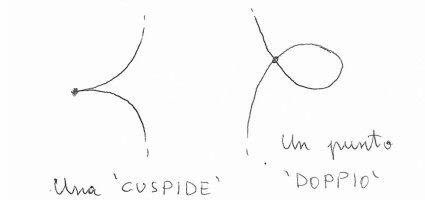
\includegraphics[width=20em]{punti-singolari.jpeg}
\curvegraph{y**2 - x**3 - x**2}{[-2:2]}{[-2:2]}

\textit{Algebricamente}, un punto $p$ zero di $f$ è singolare se $\partial_{x_i}f(p)=0$ per $i=0,\ldots,n$ (ha il differenziale nullo). \notamargine{Se il campo ha caratteristica 0, notare che $\partial_{x_i}f(p) = 0$ per ogni $i$ implica $f(p)=0$ per il \href{https://it.wikipedia.org/wiki/Funzione_omogenea}{teorema di eulero} sulle funzioni omogenee.}


\section{Cubiche, forma di Weierstrass}
Nel caso speciale di $n=2$, $\chr \bbK = 0$ c'è un importante risultato di classificazione delle curve non singolari. 
\notamargine{Una curva si dice non singolare se ogni suo punto è non singolare.} 

Consideriamo curve descritte da
$$ zy^2= ax^3+bx^2z+cxz^2+dz^3 $$
 dove $ax^3+bx^2+cx+d$ è un polinomio senza radici multiple, detta \smallcaps{forma di weierstrass}. Allora è non singolare. Imponiamo infatti le tre equazioni:

%% ESERCIZIO: dimostrare che la forma di weierstrass è non singolare

$$ \left\{ 
\begin{matrix}
&3ax^2&+2bxz&+cz^2 & = & -\partial_{x}f & = 0 \\
&&yz& & = & \partial_{y}f / 2 &= 0 \\
y^2 &-bx^2&-2cx&-3dz^2 & = & \partial_{z}f& = 0 \\
ax^3&+bx^2z&+cxz^2&+dz^3& = & zy^2&
\end{matrix}
\right.$$

Dalla (2) abbiamo due casi:

\begin{itemize}
	\item Se $z=0$ allora (4) dà $x=0$ e dunque $y=0$ dalla (3), assurdo.
	\notamargine{ Siamo nel proiettivo: $x=y=z=0$ non è un punto!} 

	\item Se $y = 0$, $z \neq 0$ allora (4) dà $q(x/z) = 0$ e (1) dà $q'(x/z) = 0$ (dove $q$ è il polinomio di coefficienti $a,b,c,d$). Ma allora $x/z$ sarebbe una radice multipla di $q$, assurdo.  
	\notamargine{Infatti vale il criterio della derivata, cioè un polinomio $p$ ha radici multiple se e solo se $p$ e $p'$ hanno un fattore in comune.}
\end{itemize}

Viceversa, data una curva cubica non singolare, può essere descritta da un polinomio in forma di weierstrass. Algebricamente, per ogni polinomio omogeneo $f$ di grado 3 con differenziale mai nullo, esiste una $L \in \bbP GL_2(\bbK) $ tale che $f \circ L$ (che è ancora un polinomio omogeneo di grado 3) è in forma di Weierstrass. 
\paragraph{IDEA}. Si dimostra che esiste un punto di flesso, e poi si considera una proiettività che manda il punto di flesso nel punto all'infinito. A quel punto, con pochi conti, si arriva alla forma di Weierstrass.
\notamargine{Un punto sulla cubica è di flesso se è un punto non singolare e la tangente ha ordine di contatto $>2$. Notare che nella forma di Weierstrass $(0:1:0)$ è un punto di flesso}

\section{Cubiche, struttura di gruppo}

Sia $\bbK$ algebricamente chiuso. Osserviamo che presi due punti $P,Q$ su una cubica $\gamma$ e tracciata la retta $r$ per $P,Q$, essa interseca $\gamma$ esattamente in un altro punto $R:=P * Q = Q*P$. \notamargine{Vedi il \href{https://en.wikipedia.org/wiki/B\%C3\%A9zout's_theorem}{Teorema di Bezòut}.}

Fissata un'origine $O \in \gamma$, si può dimostrare che l'operazione $(P,Q) \mapsto P \cdot Q = O*(P*Q)$ rende $\gamma$ un gruppo (banalmente) abeliano. Il cambio dell'origine dà luogo a un gruppo isomorfo. Infatti se $O,O'$ sono due origini diverse, detto $O'' = O*O'$, la mappa $P \mapsto O'' * P$ è l'isomorfismo cercato:
\notamargine{Solitamente, nella forma di weierstrass, si prende $O=(0:1:0)$, il punto all'infinito.}
$$ O'' * (P \cdot' Q) = O'' * O'*P*Q = O*P*Q $$
$$ (O''*P) \cdot (O''*Q) = (O*O'')*(P*O'')*Q = O'*O''*P*Q=O*P*Q$$

%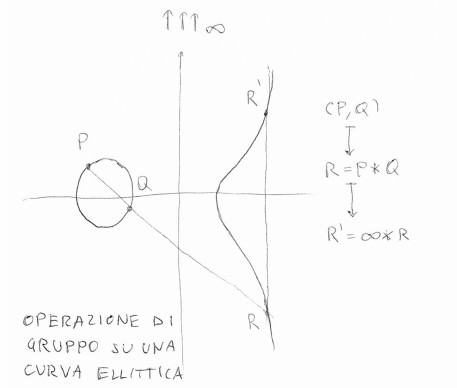
\includegraphics[width=16em]{gruppo-cubica.jpeg}

L'associatività è la proprietà più impegnativa da dimostrare. Vale la pena di notare che l'operazione è una funzione razionale delle coordinate dei punti. 
\section{Funzioni ellittiche, curve ellittiche, reticoli}
C'è una stretta correlazione tra reticoli\notamargine{Per reticoli, dove non diversmaente specificato, intendermo reticoli di rango 2 nel piano complesso}, funzioni ellittiche, curve ellittiche.

Dato un reticolo $L$, saremo in grado di costruire una funzione olomorfa con gruppo dei periodi L detta $\wp_L$.
D'altronde, questa speciale funzione ellittica $\wp_L$ rispetta $\wp_L'(z)^2= f_L(\wp_L(z))$ per un opportuno polinomio di terzo grado $f_L$. Perciò, la funzione $\varphi_L: z \mapsto (\wp_L'(z), \wp_L(z) )$ parametrizza una cubica $E_L$.

\begin{diagram}
 \bbC & \rTo & E_L \\
 \dTo &  \ruTo    & \\
 \bbC/L & &  \\
\end{diagram}
 
\section{Moduli}
Vogliamo cercare ora uno 'spazio dei parametri' per i tori complessi. Conosciamo già una parametrizzazione ridondante: dato un reticolo discreto $L=\omega_1 \bbZ + \omega_2 \bbZ$ possiamo costruire il toro $\bbC / L$ ( e tutti i tori sono definiti così), con $\omega_1, \omega_2$ non paralleli (ossia $\omega_1/\omega_2$ non reale). Cerchiamo ora di eliminare la ridondanza della parametrizzazione, partendo da $\mathcal{A} = \{ (\omega_1, \omega_2) \in \bbC^2: \Im(\omega_1/\omega_2) \neq 0 \} $. 

\begin{enumerate}
\item (orientazione) Anzitutto, a meno di scambiare $\omega_1, \omega_2$, possiamo supporre che $\Im(\omega_1/\omega_2) > 0$: infatti se fosse negativa, $\Im(\omega_2/\omega_1) = -\Im(\omega_1/\omega_2)  > 0$ sarebbe positiva.
\item (riscalamento) Se $\lambda \in \bbC^*$, allora $\bbC/\lambda L  \simeq \bbC/L$ tramite la mappa $z \mapsto \lambda z$ da $C/L$ in $C/\lambda L$. Dunque se $L= \omega_1\bbZ + \omega_2 \bbZ$ con $\Im(\omega_1/\omega_2) > 0$ possiamo considerare $\omega_2^{-1}L= \tau \bbZ + \bbZ $ con $\Im \tau > 0$. Ora il nostro spazio dei parametri perciò è $\mathcal{H} = \{ \tau \in \bbC: \Im \tau > 0 \} \simeq \mathcal{A} / \text{omotetie}$. Se $(\omega_1, \omega_2) \in \mathcal{A}$ indichiamo con $[\omega_1, \omega_2]$ la sua classe di equaivalenza a meno di omotetie, che ha un rappresentante privilegiato $[\omega_1/\omega_2, 1]$ in $\mathcal{H}$.
\item (cambio base) Se $M$ è una matrice 2x2 a coefficienti interi e $L=\omega_1\bbZ + \omega_2\bbZ$ è un reticolo, possiamo considerare il reticolo generato da $M[\omega_1, \omega_2]$ ($M \in End(\bbZ^2) \subset End(\bbC^2)$ agisce sulle coppie di complessi). Visto che le coppie di complessi sono a meno di omotetie, possiamo considerare $M,N \in End(\bbZ^2)$ equivalenti se esiste $\lambda \in \bbC^*$ tale che $\lambda M = N$. Il gruppo delle matrici invertibili a meno di scalari si chiama $\bbP GL_2(\bbZ)$. \notamargine{In realtà, visto che $M,N$ sono a coefficienti interi, $\lambda$ deve essere razionale.} Se $M \in \bbP GL_2(\bbZ)$, allora $M[\omega_1,\omega_2]$ è equivalente a $[\omega_1,\omega_2]$, perciò lo spazio dei parametri ora è $(\mathcal{A}/\text{omotetie})/\bbP GL_2(\bbZ)$.
\item (parametrizzazione esplicita) Così come per ogni classe di equivalenza $[\omega_1, \omega_2]$ a meno di omotetie abbiamo scelto un rappresentante privilegiato $[\tau,1]$, così scegliamo per ogni matrice $[M] \in \bbP GL_2(\bbZ)$ a meno di omotetie un rappresentante privilegiato in $SL_2(\bbQ)$. Infatti $[M*M'] = \mathrm{ Id} $ significa che esiste $\lambda \in \bbC^*$ tale che
$[M]*[M'] = \lambda \mathrm{Id} $. In particolare $\mathrm{det } M$ è invertibile, perciò possiamo scegliere $(\mathrm{det }M)^{-1}M$ equivalente a $M$ e condeterminante 1 ( e ha coefficienti in $\bbQ$). Se prendiamo ora $M \in SL_2(\bbQ)$ di coefficienti $a,b,c,d$ e lo facciamo agire su $[\tau,1]$ otteniamo $\displaystyle [a\tau+b,c\tau+d]= \left [ \frac{a\tau+b}{c \tau + d}, 1 \right ] $ .\notamargine{e si può verificare che  $\frac{a\tau+b}{c \tau + d}$ ha ancora parte immaginaria positiva.} Perciò $SL_2(\bbQ)$ agisce su $\mathcal{H}$ tramite $ M( \tau) = \frac{a \tau+b}{c\tau+d} $, e il nostro spazio dei parametri diventa infine $\mathcal{H} / SL_2(\bbQ)$.
\end{enumerate}

Dimostreremo nelle prossime lezioni che questa parametrizzazione non è più ridondante: se due tori hanno parametri diversi, allora \textit{non} sono biolomorfi. Questo seguirà dalla classificazione esplicita delle funzioni olomorfe tra tori (vedi lezione sulle isogenie).



\end{document}

